\section{A bounded-reward Gaussian construction}
\label{app:gaussian}

The finite-action analysis isolates the role of the score space. The following construction shows that positive weighting can also reverse the mean update of a scalar Gaussian actor.

\begin{proposition}[Direction reversal for a continuous actor]
\label{prop:gaussian}
Let $Z\sim\mathcal N(\theta,1)$ and let
\[
r(Z)=\sin Z-\sin(2Z)-2,\qquad
w(Z)=\frac1{50}+\frac{49}{50}e^{-Z^2}.
\]
At $\theta=0$, use the exact advantage and hold $w$ fixed in the surrogate derivative. Then the expected-return gradient is positive and the weighted score gradient is negative. The conclusion also holds for the bounded action $a=2\tanh Z$, with the reward and weight expressed through $Z=\operatorname{atanh}(a/2)$. If the actor also learns its log standard deviation $\eta$, the full two-parameter gradient reverses at $(\theta,\eta)=(0,0)$.
\end{proposition}

\begin{proof}
The reward lies in $[-4,0]$. Symmetry gives $\E r=-2$ at $\theta=0$, so the exact advantage is $A(Z)=\sin Z-\sin(2Z)$. The score for the Gaussian mean is $Z$ there. Differentiating its characteristic function gives
\[
\E[Z\sin(kZ)]=ke^{-k^2/2}.
\]
The derivative is justified by $\E|Z|<\infty$. Completing the square in the Gaussian integral gives
\[
\E[e^{-Z^2}Z\sin(kZ)]
=\frac{k}{3\sqrt3}e^{-k^2/6}.
\]
Consequently,
\begin{align}
g&=e^{-1/2}-2e^{-2}>0,\\
g_w&=\frac1{50}g+
\frac{49}{150\sqrt3}\left(e^{-1/6}-2e^{-2/3}\right).
\label{eq:gaussian-gradient}
\end{align}
The first sign uses $e^{3/2}>2$. To check the second sign with explicit bounds, the alternating Taylor bounds for $e^{-x}$ on $0<x<1$ give
\[
2e^{-2/3}-e^{-1/6}
\ge 2\left(1-\frac23+\frac29-\frac4{81}\right)
-\left(1-\frac16+\frac1{72}\right)
=\frac{107}{648}.
\]
Since $g<1$ and $\sqrt3<2$,
\[
g_w<\frac1{50}-\frac{49}{300}\frac{107}{648}<0.
\]
For differentiating the expected reward in $\theta$, the reward is bounded and the Gaussian density derivative on a bounded neighborhood of zero has an integrable Gaussian envelope times a linear factor. Dominated convergence therefore identifies $g$ with the derivative of the expected return.

For the family $Z\sim\mathcal N(\theta,e^{2\eta})$, the log-scale score at $(0,0)$ is $Z^2-1$. Differentiation in $\eta$ is justified by a Gaussian envelope times a quadratic factor. The advantage is odd, and the weight and log-scale score are even. Both the unweighted and weighted log-scale gradients therefore vanish. The full gradients are $(g,0)^\top$ and $(g_w,0)^\top$, whose inner product is negative.

Under $a=2\tanh Z$, the density Jacobian at a fixed action is independent of both parameters, so the scores are unchanged. The same expectations and signs apply. Values assigned to the reward at $a=\pm2$ have probability zero and can be chosen in $[-4,0]$.
\end{proof}

The weight satisfies $0.02<w\le1$ and can be written in the form of \eqref{eq:implemented-weight}: choose $u(z)=-(\tau_u/\beta)\log w(z)$ with $\beta,\tau_u>0$. This represents an admissible fixed confidence signal. The construction analyzes the weighting operation; the signal is specified analytically.

\section{The local PPO derivative and advantage centering}
\label{app:ppo}

Let $\theta_0$ be the reference policy, and hold sampled advantages and weights fixed. For a finite action space, define the exact expected clipped surrogate
\[
L_w(\theta)=\E_{p}\min\left\{\rho_\theta wA,\operatorname{clip}(\rho_\theta,1-\epsilon,1+\epsilon)wA\right\}.
\]
Here $\rho_\theta=\pi_\theta/\pi_{\theta_0}$ and $\epsilon>0$.

At $\theta=\theta_0$, every ratio equals one. Full support and differentiability give a neighborhood in which all finitely many ratios lie inside the clipping interval. Thus
\begin{equation}
\nabla L_w(\theta_0)=\E_p[wA\psi]=g_w(A).
\end{equation}
This equality concerns the initial expected surrogate derivative. A positive common rescaling of exact centered advantages preserves its direction.

Extending the weighted score sum to all advantage vectors, for an arbitrary centering constant $c$,
\begin{equation}
g_w(A-c)=g_w(A)-c\E_p[w\psi].
\label{eq:weighted-baseline}
\end{equation}
Action-dependent weights can therefore make the choice of center affect the update. Related baseline and score-centering effects are analyzed in \cite{tucker,han}. In the experiments, centering and scaling use each minibatch, the critic provides GAE estimates, and PPO performs several Adam updates. The exact local analysis identifies the expected weighting operation before those additional choices.

\section{The stronger-policy comparison}
\label{app:strong-policy}

\begin{table}[htbp]
\centering
\small
\caption{Refinement from the stronger policy, with one run per method. Values are means $\pm$ sample standard deviations across 50 matched evaluation episodes. Each episode has 200 steps. These spreads describe episodes within a checkpoint.}
\label{tab:strong-policy}
\begin{tabular}{lrrr}
\toprule
Method & Environment return & Return gap & Final length\\
\midrule
Starting policy & $-150.47\pm86.30$ & $-0.12\pm0.55$ & ---\\
Fixed $H=5$ & $-295.68\pm294.85$ & $2.03\pm8.19$ & $5.00$\\
Fixed $H=20$ & $-149.74\pm86.59$ & $-0.19\pm0.40$ & $20.00$\\
Uncertainty termination & $-149.83\pm86.96$ & $-0.20\pm0.48$ & $16.40$\\
Weighted advantage & $-288.62\pm282.46$ & $9.75\pm25.40$ & $20.00$\\
\bottomrule
\end{tabular}
\end{table}

\begin{figure}[htbp]
\centering
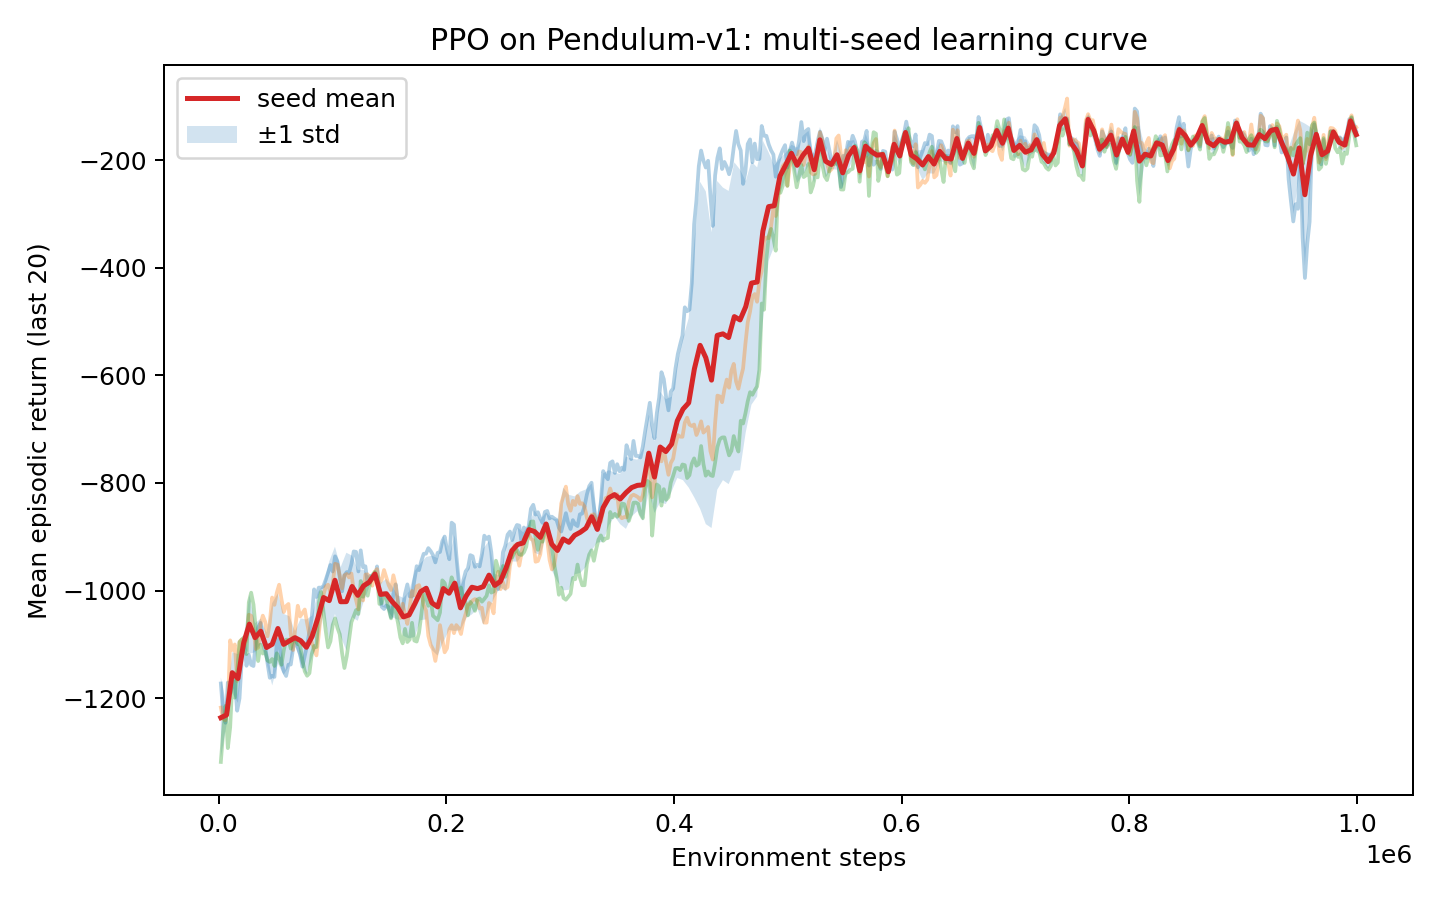
\includegraphics[width=0.84\linewidth]{images/learning_curve_mean_std.png}
\caption{Training curves for the three original PPO seeds. The deterministic evaluation means are $-148.7$, $-152.7$, and $-157.5$.}
\label{fig:ppo}
\end{figure}

\section{Code and result sources}

The repository at \url{https://github.com/TanhJK728/reliable-world-model-rl} contains the implementation and the recorded result tables. The analysis maps to the following components:

\begin{center}
\small
\begin{tabular}{p{0.39\linewidth}p{0.55\linewidth}}
\toprule
Component & Role in this paper\\
\midrule
\code{imagined\_env.py} & Segment stopping, exact reward, successor state, and reset rule.\\
\code{train\_imagined\_ppo.py} & Boundary masking in GAE and positive weights applied after advantage centering.\\
\code{ppo\_core.py} & Gaussian actor, action-density transformation, and reward function.\\
\code{world\_model.py} & Memberwise state projection, averaging, and disagreement.\\
\code{compare\_imagined\_methods.py} & Model and environment evaluation from matched starts.\\
\code{aggregate\_comparison.py} & Stored summaries across refinement seeds.\\
\bottomrule
\end{tabular}
\end{center}

\begingroup\raggedright\small
Table~\ref{tab:refinement} uses the recorded summary in \path{runs/comparison_seeds/comparison_aggregated.csv}. Table~\ref{tab:strong-policy} uses \path{runs/comparison/comparison.csv}. Prediction measurements come from \path{runs/world_model_eval/one_step_results.csv} and \path{runs/world_model_eval/rollout_results.csv}. PPO evaluation comes from \path{runs/ppo_summary/evaluation.csv}. These records provide the numerical sources for the tables and figures in this paper.
\par\endgroup
